\documentclass[../hw6.tex]{subfiles}

\begin{document}

\subsection*{46}
A hole is drilled through the center of a ball of radius $r$, leaving a solid with a hollow cylindrical core of height $h$. Show that the volume of this solid is independent of the radius of the ball.

This volume is known as a napkin ring.

We will consider both $r,h$ to be non-negative.

We take a cross section of the ball to examine the relationship between $r$ and $h$.

\begin{figure*}[ht]
\centering    
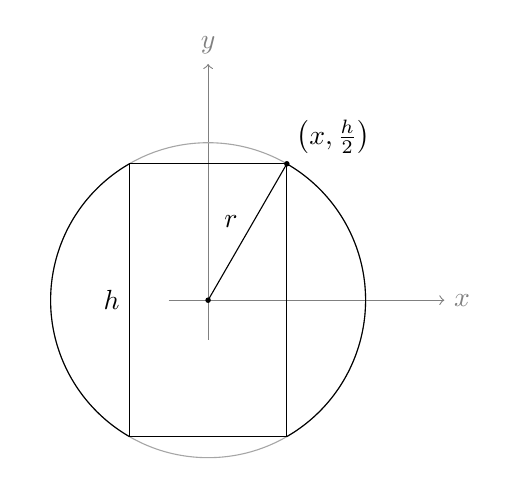
\begin{tikzpicture}
    \draw[->, gray] (0,-0.5) -- (0,3) node[above] {$y$};
    \draw[->, gray] (-0.5,0) -- (3,0) node[right] {$x$};

    \draw (0,0) -- (1,{sqrt(3)}) node[above right] {$\left( x, \frac{h}{2} \right)$};
    \node[left] at (0.5,1) {$r$};
    \draw[gray!70] (0,0) circle (2);
    \draw (-1,{sqrt(3)}) arc (-60:60:-2);
    \draw (1,-{sqrt(3)}) arc (-60:60:2);
  
    \fill (0,0) circle[radius=1pt];
    \fill (1,{sqrt(3)}) circle[radius=1pt];

    \node[left] at (-1,0) {$h$};
    \draw (-1,{-sqrt(3)}) rectangle (1,{sqrt(3)});
\end{tikzpicture}  
\end{figure*}

We see that, \[r^2=x^2+{\left( \frac{h}{2} \right)}^2.\]

From this relationship, we can see that the height of the cylinder $h$ is, \[h=2\sqrt{r^2-x^2}.\]

Likewise, we also see that the radius of the cylinder, equal to $x$, which we will call $R$, is \[R=\sqrt{r^2-\frac{h^2}{4}}.\]

We will form the volume of the napkin ring by a solid of revolution from the portion of the ball to the right of the $y$-axis on positive $x$. Thus the bounds of integration are $x\in[R,r]$.

We integrate using the cylindrical shells, noting that the height of each shell is the total height of the ball, or $h=2\sqrt{r^2-x^2}$, and the circumference is $2\pi x$.

We will also use a substitution with the function $u(x) = r^2-x^2$. We see that $du=-2xdx$, $u(r)=r^2-r^2=0$, and $u(R)=r^2-{\sqrt{r^2-\frac{h^2}{4}}}^2=\frac{h^2}{4}$.
\begin{align*}
    V &= \int_{R}^{r} 2\pi x \left( 2\sqrt{r^2-x^2} \right) dx \\
    &= 4\pi \int_{R}^{r} x \sqrt{r^2-x^2} dx \\
    &= \frac{4\pi}{-2} \int_{R}^{r} {-2x} \sqrt{r^2-x^2} dx \\
    &= {-2\pi} \int_{u(R)}^{u(r)} \sqrt{u} \, du \\
    &= {-2\pi} \left[ \frac{2}{3} u^{\frac{3}{2}} \right] \Bigg\vert_{\frac{h^2}{4}}^{0}.
\end{align*}

We can immediately see that the volume will not depend on $r$ without further computation.

Still,
\[V = -2\pi\left( -\frac{2}{3} {\left( \frac{h^2}{4} \right)}^{\frac{3}{2}} \right) = \frac{4\pi}{3} \left( \frac{h^3}{8} \right) = \frac{h^3\pi}{6}.\]

Thus, the volume of the napkin ring only depends on the height of the cylindrical core.

\end{document}